\chapter{REFERENCIAL TEÓRICO}

Neste capítulo é feita uma revisão de assuntos relacionados, visando embasamento conceitual, para o entendimento deste trabalho.

\section{Equipamentos de pequeno porte}

No mundo atual podemos encontrar diversos tipos de computador. Existem os de grande porte, conhecidos como \textit{mainframes}, os de médio porte, como os servidores e \textit{workstations}, e os de pequeno porte, que podem ser divididos em duas categorias: os de mesa (\textit{desktops}) e os portáteis (\textit{notebooks}).

Os tipos de computadores citados no parágrafo anterior são utilizados a partir da necessidade de cada usuário. \textit{Mainframes}, por exemplo, são usados para processar um grande volume de informações, enquanto que \textit{desktops} ou \textit{notebooks} atendem à demandas que exigem um menor poder de processamento.

Dessa forma, existindo diferenças nos objetivos de uso de cada equipamento, e também uma disparidade considerável entre os custos dos mesmos, os minicomputadores estão entre os mais utilizados nos dias atuais, pois têm um custo acessível e atendem às necessidades dos usuários comuns de forma eficiente. Até empresas poderiam conter gastos, sem deixar a desejar na qualidade do serviço prestado, se substituíssem computadores de grande porte por outros de pequeno porte. Essa iniciativa contemplaria o cenário de uma técnica chamada \textit{downsizing}.

\section{\textit{Downsizing}}

Na área da informática o termo \textit{downsizing} define uma situação onde sistemas originalmente hospedados em um computador de grande porte (\textit{mainframe}) são adaptados para computadores de menor porte (mini/microcomputadores), e esse processo consiste em função da redução do porte da empresa ou do aumento da capacidade computacional dos computadores de menor custo \cite{WIKIPEDIA3}.

\section{\textit{Thin client}}

O \textit{thin client} é um equipamento que funciona como um mini PC, mas não possui, em sua estrutura interna, HD, processador e memória (não como os convencionais). Apesar de sua estrutura simples, com ele é possível obter uma rede de baixo custo e de fácil manutenção, dentre outros benefícios \cite{THINCLIENT}.

\begin{figure}[ht]
    \centering
    \scalebox{0.7}{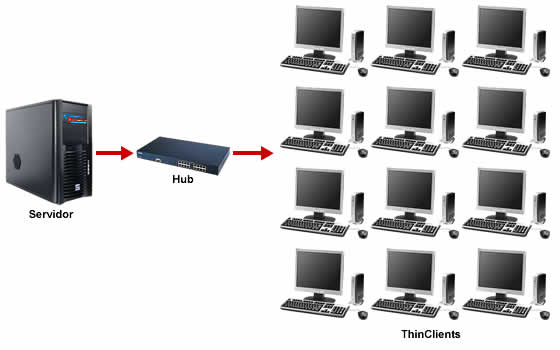
\includegraphics{figuras/rede_thin_clients}}
    \caption{Representação de uma rede de computadores com \textit{thin clients}.}
\end{figure}

Com a implantação de \textit{thin clients} e apenas um computador (\textit{host} ou servidor) é possível gerar várias estações de acesso. A configuração do servidor depende do número de terminais e das necessidades dos usuários da rede. Esta deve ser bastante pensada antes de elaborar e formatar o ambiente utilizado.

Vale a pena acrescentar aqui uma relação entre a formas de funcionamento dos equipamentos \textit{thin client} e de sistemas informatizados desenvolvidos para a \textit{web}. Assim como um \textit{thin client} utiliza os recursos de um servidor configurado, um sistema \textit{web} ao ser executado também utiliza os recursos do servidor no qual está hospedado. Dessa forma, mesmo que o computador do usuário final tenha recursos limitados, todo o processamento relacionado às funcionalidades do sistema será realizado no servidor.

No estudo de caso que será efetuado neste trabalho, o \textit{Raspberry Pi} irá respeitar esse modelo de processamento, pois o sistema criado para gerenciar as demandas do setor alvo da pesquisa foi desenvolvido utilizando arquitetura \textit{web}. Dessa forma é claramente possível de se notar o quanto a evolução tecnológica torna os equipamentos de mesa mais acessíveis para o consumidor.

\section{Barateamento dos equipamentos de mesa}

Atualmente, sob a ótica financeira, comprar um computador não é mais uma tarefa impossível, mas há alguns anos os preço desses equipamentos eram muito pouco acessíveis. Chega a ser difícil crer que a cerca de 15 anos o valor pago por um computador com configurações totalmente inferiores às dos computadores atuais, era de R\$ 4 mil, aproximadamente \cite{HAMANN}.

Para se entender o por quê dos altíssimos preços desses equipamentos, é preciso atentar-se para o ciclo de vida das tecnologias. Aparelhos que custam muito têm seus valores reduzidos gradativamente até que cheguem aos preços mais populares, então surgem novas tecnologias, fazendo com que a curva dos preços volte a subir e o ciclo se repita. Isso pode ser percebido com televisores e suas diferentes tecnologias: CRT, LCD, Plasma, LED e os novos modelos 3D que ainda estão com preços altíssimos \cite{HAMANN}.

Em se tratando de informática, não é diferente. Os componentes de hardware sempre são lançados com valores altos que, com o passar do tempo, são reduzidos. Um dos fatores que mais contribui para a redução nos preços é a evolução tecnológica, pois quando são lançados novos produtos, é necessário reduzir os valores dos mais antigos para que eles não fiquem presos nas fábricas \cite{HAMANN}. Essa maior acessibilidade provocada pela evolução técnológica pode ser muito útil quando se observa o cenário das pequenas empresas no Brasil e no mundo.

\section{Realidade brasileira de pequenas empresas como maior categoria de empresas no Brasil e no mundo}

Todas as informações apresentadas nesta seção são de \citeonline{PORTALBRASIL}.

As pequenas e médias empresas (MPEs) são fundamentais para promover o crescimento econômico, criar empregos e renda e melhorar as condições de vida da população. Os indicadores desse segmento empresarial demonstram sua importância na economia, não só no Brasil, mas em todo o mundo.

A contribuição das MPEs é reconhecida principalmente na capilaridade que estes negócios propiciam e na absorção de mão de obra, inclusive aquela com maior dificuldade de inserção no mercado, como jovens em busca pelo primeiro emprego e as pessoas com mais de 40 anos. As pequenas empresas também são capazes de dinamizar a economia dos municípios e bairros das grandes metrópoles.

“Pequenas empresas são o sustentáculo de uma economia em qualquer lugar do mundo. São elas que agregam valor a produtos e serviços”, afirma o diretor executivo do Centro de Inovação, Empreendedorismo e Tecnologia (Cietec), incubadora de empresas da Universidade de São Paulo (USP), Sérgio Risola. Segundo dados mais recentes do IBGE, as MPEs representam 20\% do Produto Interno Bruto (PIB) brasileiro, são responsáveis por 60\% dos 94 milhões de empregos no país e constituem 99\% dos 6 milhões de estabelecimentos formais existentes no país. A maior parte dos negócios estão localizados na região Sudeste (com quase 3 milhões de empresas) e o setor preferencial é o comércio, seguido de serviços, indústria e construção civil.

Desde 2000, a participação das MPEs no total de empreendimentos produtivos brasileiros aumentou bastante. Enquanto a taxa de crescimento anual foi de 4\% para o total de empresas, independente do porte, para as pequenas empresas foi de 6,2\%, e 3,8\% para as micro, entre 2000 e 2008. Nesse mesmo período, as MPEs foram responsáveis por aproximadamente metade dos postos de trabalho formais criados, ou seja, 4,5 milhões de empregos.

O faturamento das MPEs também cresceu consideravelmente nos últimos anos. No primeiro semestre de 2010, a receita real registrou aumento de 10,7\% comparado ao mesmo período de 2009. Este indicador aponta que as pequenas empresas superam o ritmo de crescimento da economia brasileira. Essa é a maior taxa de crescimento de faturamento desde que o Sebrae iniciou a pesquisa, em 1998.

\begin{table}[!htpb]
 \centering
    \begin{tabular}{|l|p{5cm}|c|} 
    \hline
        \textbf{As MPEs no Brasil} & \textbf{O que isso representa} \\
    \hline
        20\% do PIB & R\$ 700 bilhões \\
    \hline
        99\% das empresas & R\$ 5,7 milhões de MPEs \\
    \hline
        60\% dos empregos & R\$ 56,4 milhões de empregos \\
    \hline
    \end{tabular}
    \caption{Estatísticas das MPEs no Brasil}
    \label{t_fixa}
\end{table}